\documentclass[11pt,a4paper,twoside,german]{article}
\usepackage[absolute]{textpos}
\usepackage[dvipsnames]{xcolor}
\usepackage{xcolor}
\usepackage{enumitem}
\usepackage{framed}
\usepackage{epsfig}
%\usepackage[latin1]{inputenc}
\usepackage[utf8]{inputenc}
\usepackage{lscape}
\usepackage{german}
%\usepackage{graphicx}
\usepackage{graphics}
\usepackage{listings}
\usepackage[T1]{fontenc}
\usepackage{amsmath, amsfonts, amssymb}
\usepackage{textcomp}
\usepackage[official,right]{eurosym}
\usepackage{hyperref}
%\usepackage[version=3]{mhchem}
%\usepackage{epic,carom}
%\usepackage{rsphrase}
\usepackage{chemfig}
\usepackage{framed}
\usepackage{graphicx}
\usepackage{url}
\usepackage{cite}
\usepackage{ngerman,latexsym,t1enc}
\usepackage[font=small,labelfont=bf]{caption}
\usepackage{wrapfig}
\usepackage{lmodern}
\usepackage{blindtext}
%\usepackage{pgfbaseimage}
\usepackage{epstopdf}
\usepackage{color}
\usepackage{tabularx, tabulary}
\usepackage{booktabs}
\usepackage{multirow}
%\usepackage{mathtools}
\usepackage{ulem}


% === kleine Bleistifte, Blumen und solches Zeug ===
\usepackage{bbding}
\usepackage{pifont}

\usepackage{array}
\usepackage{longtable}
%\usepackage{dingbat}

%\usepackage{booktabs}
%\usepackage[pdf]{pstricks}
% \usepackage{ifpdf}
% \usepackage{verbatim}
% \usepackage[active,tightpage]{preview}
\usepackage{tikz}
\usepackage{tikz-3dplot}
\usetikzlibrary{positioning,shapes,shadows,arrows,arrows.meta,shapes.multipart,lindenmayersystems,decorations.fractals,decorations.footprints,calc,intersections,through,backgrounds,petri,decorations}
\usetikzlibrary{decorations.markings,decorations,fit,scopes,arrows,calc,shapes.misc,shapes.arrows,chains,matrix,positioning,decorations.pathmorphing,shapes,backgrounds,decorations.text}
\usetikzlibrary{arrows}
\usetikzlibrary{decorations}
\usetikzlibrary{through}
\usetikzlibrary{angles}
\usetikzlibrary{patterns}
% === Smilies und solches Zeug ===
\usepackage{tikzsymbols}

\usepackage{times}
\usepackage{exscale} % Anpassung mathematischer Symbole an aktuelle Schriftgröße
\usepackage{pgfplots}

\pagestyle{myheadings}
\parindent0em
\parskip1.5ex plus1ex minus0.5ex
\textheight25cm \textwidth16cm \evensidemargin-0.5cm
%\textheight50cm \textwidth32cm \evensidemargin-0.1cm
\topmargin-2cm \headheight1cm \headsep0.5cm %\mathindent4cm

\pagenumbering{arabic}

\tikzset{
    state/.style={
           rectangle,
           rounded corners,
           draw=black, very thick,
           minimum height=2em,
           inner sep=2pt,
           text centered,
           },
}


\begin{document}
Timo schreibt in einer ganz bestimmten Reihenfolge Zahlen in das Quadratgitter. Welche Zahlen werden in den Kästchen A, B und C stehen, wenn Timo fertig ist?
\begin{center}
	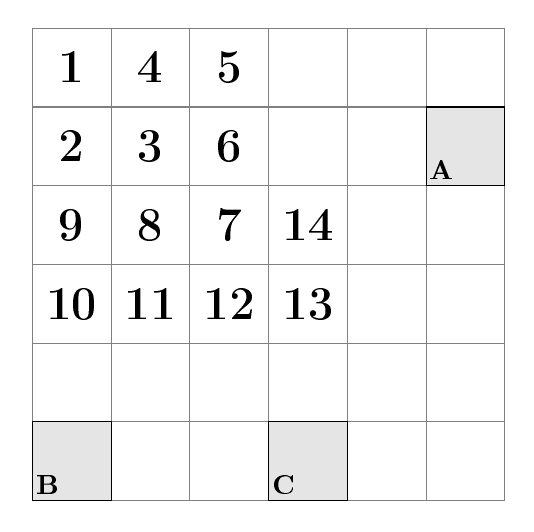
\begin{tikzpicture}
	\draw[color=gray] (0,0) grid[xstep=1cm, ystep=1cm] (6,6);
	\node at (0.5,5.5) {\LARGE \bf 1};
	\node at (0.5,4.5) {\LARGE \bf 2};
	\node at (1.5,4.5) {\LARGE \bf 3};
	\node at (1.5,5.5) {\LARGE \bf 4};
	\node at (2.5,5.5) {\LARGE \bf 5};
	\node at (2.5,4.5) {\LARGE \bf 6};
	\node at (2.5,3.5) {\LARGE \bf 7};
	\node at (1.5,3.5) {\LARGE \bf 8};
	\node at (0.5,3.5) {\LARGE \bf 9};
	\node at (0.5,2.5) {\LARGE \bf 10};
	\node at (1.5,2.5) {\LARGE \bf 11};
	\node at (2.5,2.5) {\LARGE \bf 12};
	\node at (3.5,2.5) {\LARGE \bf 13};
	\node at (3.5,3.5) {\LARGE \bf 14};

	\draw[fill=gray!20] (5,4) rectangle (6,5);
	\draw[fill=gray!20] (0,0) rectangle (1,1);
	\draw[fill=gray!20] (3,0) rectangle (4,1);
	\node at (5.2,4.2) {\bf A};
	\node at (0.2,0.2) {\bf B};
	\node at (3.2,0.2) {\bf C};
	\end{tikzpicture}
\end{center}
\end{document}